%\thispagestyle{myheadings}
\newpage
\section{Keynote Speaker: Alexis Palmer}
\setheaders{Keynote Speaker}{\daydateyear}
\index{Palmer, Alexis}

\begin{center}
{\bfseries\Large A tricky intersection: Natural language processing\\\vspace{2.0\lineskip} and endangered language documentation} \\
\vspace{1.0em}
{\large\bf Alexis Palmer} \\
University of Colorado Boulder

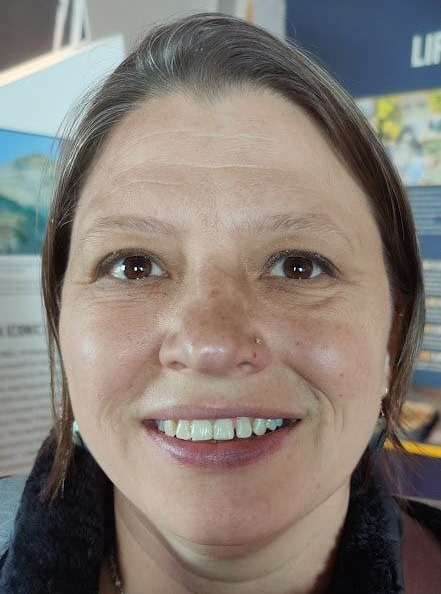
\includegraphics[width=0.4\linewidth]{content/mexican_nlp/palmer.png}

\textbf{\daydateyear{}, 10:00--11:00 CST}\\
\textbf{Do\~na Adelita}
\end{center}

\noindent
{\bfseries Abstract:}
Of the roughly 7000 languages spoken across the globe, more than half have been categorized as endangered, threatened, or of decreasing vitality. Only a handful of the world’s languages have anywhere near the amount of digitally-available data needed to train large language models such as ChatGPT, leading to a dramatic disparity in access to cutting-edge technologies. At the same time, for several decades now, linguists, language activists, language community members, and other researchers have recognized language endangerment as a pressing issue and have devoted considerable time to the incredibly time-consuming work of language documentation and revitalization. And yet, as a field, we have not yet realized the potential of natural language processing (NLP) technologies to support language documentation, description, and revitalization. In this talk, I will discuss some of the structural barriers inherent to the intersection of NLP and endangered language documentation, as well as some important ethical considerations that arise at this intersection. I will also present our work on developing models to partially automate the complex linguistic analysis work involved with producing interlinear glossed text, an important format in language documentation.

\vspace{1em}

{\bfseries Biography:}
Alexis Palmer is an assistant professor in Linguistics at CU Boulder, a fellow of the ICS, and affiliated faculty with the department of Computer Science. Her primary research focus is on computational linguistics for low-resource and endangered languages. She also works in computational semantics, computational discourse, and computational analysis of toxic language. Her current work includes incorporating linguistic insights into cross-lingual transfer learning in order to more rapidly build tools to support low-resource and endangered languages. She is a member at large of the ACL Special Interest Group on Typology and Multilingual NLP, and a founding member of the ACL Special Interest Group on Endangered Languages. Alexis grew up in Northern Michigan, did her PhD at the University of Texas in Austin, and made her way to Boulder by way of several years in German universities and research institutions, as well as the University of North Texas.

\newpage
